\documentclass[12pt,a4paper,oneside]{article}
\usepackage[spanish,activeacute]{babel}
\usepackage[utf8]{inputenc}
\usepackage[left = 2.5cm, top = 2cm, right = 2.5cm, bottom = 2cm]{geometry}
\usepackage{graphicx}

\spanishdecimal{.}

\newpage\pagenumbering{arabic}
\setcounter{page}{1}

\renewcommand{\baselinestretch}{1}

\begin{document}

\part*{Anexo V}

\subsection*{Evolución de los parámetros de NNAR}

\vspace*{3\baselineskip}
\vspace*{1\baselineskip}
\begin{figure} [h]
    \centering
    \centerline{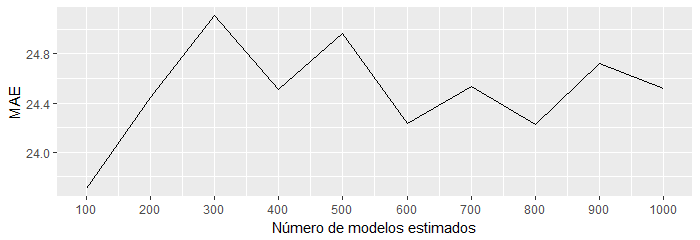
\includegraphics[scale = 0.7]{Images/modelos.png}}
    \caption{Número de modelos estimados}
    \label{red}
\end{figure}
\begin{figure} [h]
    \centering
    \centerline{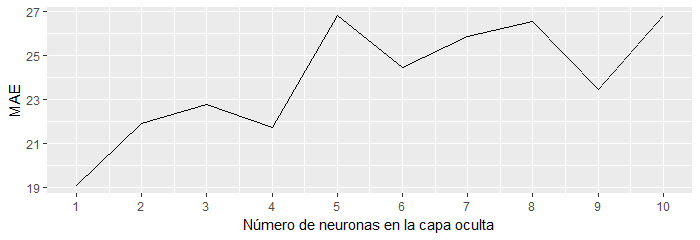
\includegraphics[scale = 0.7]{Images/neuronas.png}}
    \caption{Número de neuronas en la capa oculta}
    \label{red}
\end{figure}
\begin{figure} [h]
    \centering
    \centerline{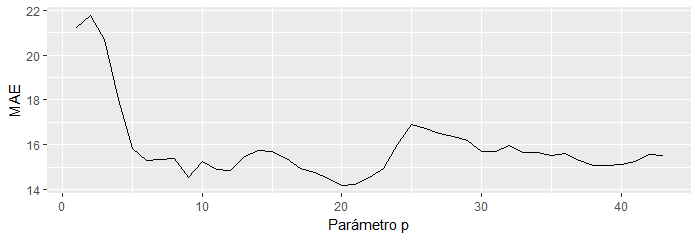
\includegraphics[scale = 0.7]{Images/p.png}}
    \caption{Parámetro p}
    \label{red}
\end{figure}
\begin{figure} [h]
    \centering
    \centerline{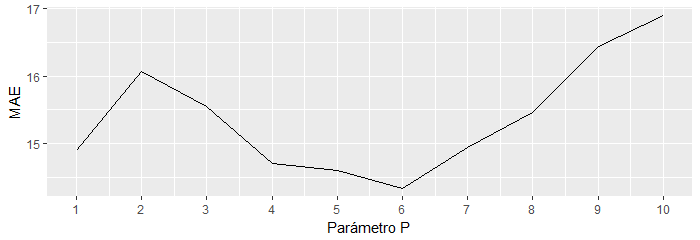
\includegraphics[scale = 0.7]{Images/PP.png}}
    \caption{Parámetro P}
    \label{red}
\end{figure}
\vspace*{3\baselineskip}
\vspace*{3\baselineskip}
\vspace*{3\baselineskip}
\vspace*{3\baselineskip}
\vspace*{3\baselineskip}

\end{document}
